\documentclass[a4paper,12pt]{report}
\usepackage[utf8]{inputenc}
\usepackage{amsmath}
\usepackage{graphicx}
\usepackage{listings}
\usepackage{tikz}
\usepackage[T1]{fontenc}
\usepackage{color}
\usetikzlibrary{arrows,automata}
\definecolor{pythonred}{rgb}{0.6,0,0} % for strings
\definecolor{pythongreen}{rgb}{0.25,0.5,0.35} % comments
\definecolor{pythonpurple}{rgb}{0.5,0,0.35} % keywords
	\definecolor{pythondocblue}{rgb}{0.25,0.35,0.75} % javadoc
	 
	\lstset{language=python,
	basicstyle=\ttfamily,
	keywordstyle=\color{pythonpurple}\bfseries,
	stringstyle=\color{pythonred},
	commentstyle=\color{pythongreen},
	morecomment=[s][\color{pythondocblue}]{/**}{*/},
	numbers=left,
	numberstyle=\tiny\color{black},
        stepnumber=2,
	numbersep=10pt,
	tabsize=4,
	showspaces=false,
	showstringspaces=false}

% Title Page

 \title{\bfseries\huge \textcolor{purple}{\underline {EEP702-Software Lab}} \\{\textcolor{blue}{Assignment6 : Dynamic Programming}}}
\author{\bfseries\large\textcolor{black}  {Harshit Kumar Gupta}\\ {\textcolor{black} {2013EET2369 }}\\

\includegraphics[width=3cm,height=3.4cm]{./iit.png}\\\noindent Computer Technology\\
\noindent Department Of Electrical Engineering\\IIT DELHI}
% iit.png: 282x282 pixel, 72dpi, 9.95x9.95 cm, bb=0 0 282 282
\begin{document}
\maketitle
\tableofcontents


\chapter{\textcolor{blue}{\underline {PROBLEM STATEMENT}}}

Problem (Compulsory - 100 marks, difficulty level: *)
 \begin{enumerate}
\item There are N packets, each with one or more candies. There are K students among 
which the packets have to be distributed. (Assume K<N for all cases). The 
parameters N and K have to be provided by the user at run-time. Each student 
gets only one packet. The number of candies in various packets are 
(x1, x2, x3,....xk ) , where xi denotes the number of candies in the ith packet.
Find the number of triplets (x1, x2, x3) possible such that sum of the candies 
(x1 + x2 + x3) is even.\\



\item Optional bonus problems:
These following problems are optional and represent higher levels of difficulty
(proportional to the number of stars **). Bonus marks (indicated against each) 
will be given for attempting these.
Let unfairness be defined.



\item Divide the packets of candies among the K students such that u is minimum
(***/10 points) Problem O2 : Divide the packets into two parts (p1 and p2) such
that the difference(|p1-p2|) is minimum, where p1 and p2 are the total number of 
candies in part 1 and part 2 respectively.
\end{enumerate}


\begin{center}
\chapter{\textcolor{blue}{\underline {ABSTRACT}}}
\end{center}
\noindent The Intention of the C++ Code is to make use of the Dynamic Programming to evalute Triplets which has even no of 
candies in the packet. In the second part we have to calculate the minimum unfairness among the packet of candies that is
to be distributed between K no of student fairly. And in the third part we have to divide the packets into two parts (p1 and p2) such that
the difference(|p1-p2|) is minimum, where p1 and p2 are the total number of candies in
part 1 and part 2 respectively.
\begin{center}
\chapter{\textcolor{blue}{\underline {INTRODUCTION}}}
\end{center}
\noindent C++ (pronounced see plus plus) is a programming language that is general purpose, statically typed, free-form, multi-paradigm and compiled. It is regarded as an intermediate-level language, as it comprises both high-level and low-level language features. Developed by Bjarne Stroustrup starting in 1979 at Bell Labs, C++ was originally named C with Classes, adding object-oriented features, such as classes, and other enhancements to the C programming language. The language was renamed C++ in 1983, as a pun involving the increment operator.

C++ is one of the most popular programming languages and is implemented on a wide variety of hardware and operating system platforms. As an efficient compiler to native code, its application domains include systems software, application software, device drivers, embedded software, high-performance server and client applications, and entertainment software such as video games. Several groups provide both free and proprietary C++ compiler software, including the GNU Project, LLVM, Microsoft and Intel. C++ has greatly influenced many other popular programming languages, most notably C and Java.

In computer science, dynamic programming is a method for solving complex problems by breaking them down into simpler subproblems. It is applicable to problems exhibiting the properties of overlapping subproblems and optimal substructure (described below). When applicable, the method takes far less time than naive methods that don't take advantage of the subproblem overlap (like depth-first search).
\begin{center}
\chapter{\textcolor{blue}{\underline {SPECIFICATIONS AND ASSUMPTIONS}}}
\end{center}
\section*{Specifications}

\begin{enumerate}
\item The parameters N and K have to be provided by the user at run-time.
\item There are K students among which the packets have to be distributed.
\item The number of candies in various packets are (x1, x2, x3,....xk ) , where xi denotes the number of candies in the ith packet.
\item Unfairness be defined as u=|sum(Xi-Xj)|.
\item Divide the packets of candies among the K students such that u is minimum

\end{enumerate}

\section*{Assumptions}

\begin{enumerate}
\item The values of N, K and No. of candies in the Packets are assumed to be one or more than one.
\item W have assumed the unfairness to be defined as u=|sum(Xi-Xj)| and u should be minimum.

\end{enumerate}
 
\begin{center}
\chapter{\textcolor{blue}{\underline {LOGIC USED/METHODOLOGY}}}
\end{center}
The methodology that is used for developing the program is defined below:\\

\begin{enumerate}
\item Input the no of packets and no of students and also the no of candies in each packet.
\item For finding the triplets with even no of candies in it, for loop is used to extract N-K set of candies and its sum is calculated.
\item If the sum is even a counter is incremented and the set's index is stored to display the triplet contents.
\item At last we get the total no of sets with even no of candies in the triplet along with the sets.
\item To calculate the unfairness we first sort the candy array in which no of candies in each packet is stored.
\item Then Following the no os students a set is made and difference of each element in the set is calculated.
\item The set with minimum difference is displayed and its minimum unfairness is also displayed.
\item For the third part sumof all the elements int the candy is taken, also sum of elements of from step-2 is also calculated.
\item The difference is calculated that gives the divided packets into two parts (p1 and p2) such that
the difference(|p1-p2|) is minimum, where p1 and p2 are the total number of candies in
part 1 and part 2 respectively.

\end{enumerate}

\begin{center}
\chapter{\textcolor{blue}{\underline {FLOWCHART}}}
\end{center}
\noindent \\Flowchart
\begin{center}
\begin{center}
 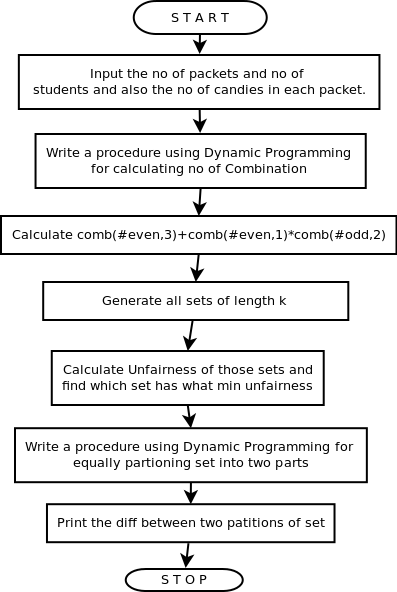
\includegraphics[width=14 cm,height=12 cm]{./Diagram1.png}
 % Diagram1.png: 658x542 pixel, 72dpi, 23.21x19.12 cm, bb=0 0 658 542
\end{center}

\end{center}

\begin{center}
\chapter{\textcolor{blue}{\underline {EXECUTION INSTRUCTIONS}}}
\end{center}
\begin{enumerate}
 \item For program following instructions are used.
 \begin{enumerate}
  \item g++ -Wall -o packet packet.cpp
\item ./packet
 \end{enumerate}

\end{enumerate}
Repeat the above instructions for different inputs.

\begin{center}
\chapter{\textcolor{blue}{\underline {RESULTS AND CONCLUSIONS}}}
\end{center}
\begin{enumerate}
 
\item For the given set of inputs the program works perfectly.
\item NO of triplets whose sum is even is counted and all triplets is printed using dynamic programming.
\item No of sets having k items is generated and  their unfairness is calculated and printed.
\item Partion of set into two set is done whose difference is minimum using dynamic programming.
\end{enumerate}



\begin{center}
 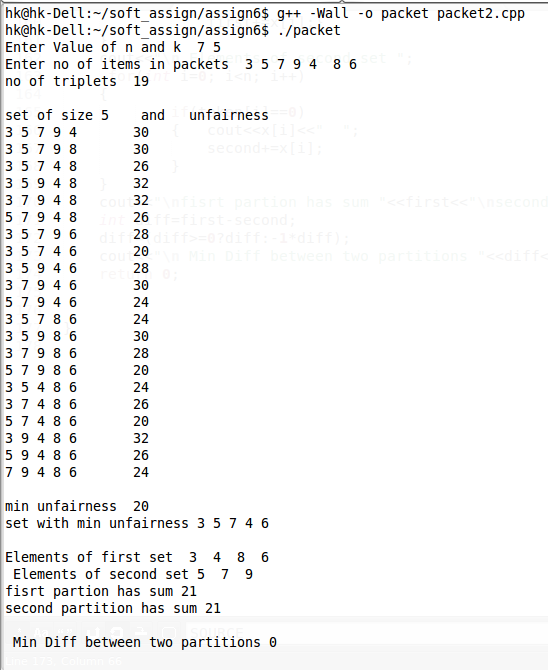
\includegraphics[width=15 cm,height=11 cm]{./output.png}
 % output.png: 1280x800 pixel, 72dpi, 45.16x28.22 cm, bb=0 0 1280 800
\end{center}

\end{document}  
